%!TEX program = xelatex
% 完整编译方法 1 pdflatex -> bibtex -> pdflatex -> pdflatex
% 完整编译方法 2: xelatex -> bibtex -> xelatex -> xelatex
\documentclass[lang=cn,11pt]{elegantpaper}
\usepackage{listings}
\usepackage{color}
\definecolor{dkgreen}{rgb}{0,0.6,0}
\definecolor{gray}{rgb}{0.5,0.5,0.5}
\definecolor{mauve}{rgb}{0.58,0,0.82}

\lstset{ %
  language=Octave,                % the language of the code
  basicstyle=\footnotesize,           % the size of the fonts that are used for the code
  numbers=left,                   % where to put the line-numbers
  numberstyle=\tiny\color{gray},  % the style that is used for the line-numbers
  stepnumber=1,                   % the step between two line-numbers. If it's 1, each line 
                                  % will be numbered
  numbersep=5pt,                  % how far the line-numbers are from the code
  backgroundcolor=\color{white},      % choose the background color. You must add \usepackage{color}
  showspaces=false,               % show spaces adding particular underscores
  showstringspaces=false,         % underline spaces within strings
  showtabs=false,                 % show tabs within strings adding particular underscores
  frame=single,                   % adds a frame around the code
  rulecolor=\color{black},        % if not set, the frame-color may be changed on line-breaks within not-black text (e.g. commens (green here))
  tabsize=2,                      % sets default tabsize to 2 spaces
  captionpos=b,                   % sets the caption-position to bottom
  breaklines=true,                % sets automatic line breaking
  breakatwhitespace=false,        % sets if automatic breaks should only happen at whitespace
  title=\lstname,                   % show the filename of files included with \lstinputlisting;
                                  % also try caption instead of title
  keywordstyle=\color{blue},          % keyword style
  commentstyle=\color{dkgreen},       % comment style
  stringstyle=\color{mauve},         % string literal style
  escapeinside={\%*}{*)},            % if you want to add LaTeX within your code
  morekeywords={*,...}               % if you want to add more keywords to the set
}



\begin{document}

\tableofcontents
\newpage

\section{中断点亮小灯}
示例程序int实现功能为中断控制控制LED灯亮,此处分析int程序
\subsection{原理分析}
利用S3C2440手册,分析解读中断初始化程序。S3C2440A 中的中断控制器接受来自 60 个中断源的请求。
提供这些中断源的是内部外设,如 DMA 控制器、UART、IIC 等等。在这些中断源中,
UARTn、AC97 和 EINTn 中断对于中断控制器而言是“或”关系。
当从内部外设和外部中断请求引脚收到多个中断请求时,中断控制器在仲裁步骤后请求
 ARM920T 内核的 FIQ或 IRQ。仲裁步骤由硬件优先级逻辑决定并且写入结果到帮助用户
 通告是各种中断源中的哪个中断发生了的中断挂起寄存器中。\\
 \\
 控制流程图如下:\\
\begin{figure}[htbp]
  \centering
  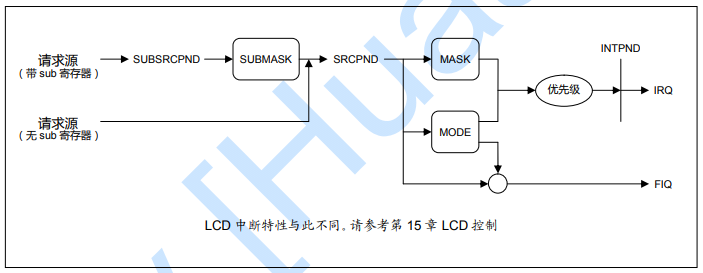
\includegraphics[width=1\textwidth]{int1.png}
  \caption{中断控制流程图}
\end{figure}
\\
1. 先收集到SRCPND\\
2. 用INTMOD判断是否为FIQ\\
3. 判断完后进入屏蔽环节INTMSK进行筛选\\
4. PRIORITY进行优先级划分\\
5. 划分结果存储在INTOFFSET\\
\\
\\
\\
\\
\\
\\
\\
原理图如下:\\
\begin{figure}[htbp]
  \centering
  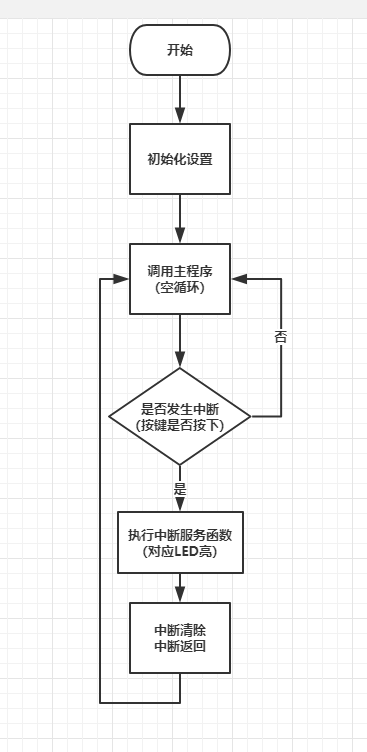
\includegraphics[width=0.3\textwidth]{sch1.png}
  \caption{中断点亮小灯原理图}
\end{figure}

\subsection{调试过程}
\subsubsection{中断初始化程序分析}
head.s程序:\\
功能:初始化,设置中断模式、管理模式的栈,设置好中断处理函数。\\
\lstset{language=bash}
\begin{lstlisting}{中断初始化程序}
  Reset:                  
  ldr sp, =4096           
  bl  disable_watch_dog   
  msr cpsr_c, #0xd2       @ 进入中断模式
  ldr sp, =3072           @ 设置中断模式栈指针

  msr cpsr_c, #0xd3       @ 进入管理模式

  bl  init_led            @ 初始化LED的GPIO管脚
  bl  init_irq            @ 调用中断初始化函数,在init.c中
  msr cpsr_c, #0x5f       @ 设置I-bit=0,开IRQ中断
  
  ldr lr, =halt_loop      @ 设置返回地址
  ldr pc, =main           @ 调用main函数
halt_loop:
  b   halt_loop
\end{lstlisting}
此段代码为中断初始化的核心,设置了中断开启的模式,并调用了各个初始化函数,如\lstinline{init_led}
和\lstinline{init_irq}

\lstset{language=bash}
\begin{lstlisting}{中断跳转程序}
HandleIRQ:
    sub lr, lr, #4                  @ 计算返回地址
    stmdb   sp!,    { r0-r12,lr }   @ 保存使用到的寄存器
                                    @ 注意,此时的sp是中断模式的sp
                                    @ 初始值是上面设置的3072
    
    ldr lr, =int_return             @ 设置调用ISR即EINT_Handle函数后的返回地址  
    ldr pc, =EINT_Handle            @ 调用中断服务函数,在interrupt.c中
\end{lstlisting}
此处为中断跳转程序,当出现特定中断时会跳转到这里,然后按照这里的指示跳转到中断服务函数,这里是跳转到
\lstinline{EINT_Handle}内。

\subsubsection{中断寄存器分析}
打开\lstinline{s3c24xx.h},这里使用到的interrupt registes,我们可以看到
\lstset{language=C}

\begin{lstlisting}{中断寄存器}
#define SRCPND              (*(volatile unsigned long *)0x4A000000)
#define INTMOD              (*(volatile unsigned long *)0x4A000004)
#define INTMSK              (*(volatile unsigned long *)0x4A000008)
#define PRIORITY            (*(volatile unsigned long *)0x4A00000c)
#define INTPND              (*(volatile unsigned long *)0x4A000010)
#define INTOFFSET           (*(volatile unsigned long *)0x4A000014)
#define SUBSRCPND           (*(volatile unsigned long *)0x4A000018)
#define INTSUBMSK           (*(volatile unsigned long *)0x4A00001c)
\end{lstlisting}
这里使用了大量中断相关寄存器。其中
SRCPND:当一个中断发生后,那么相应的位会被置1,
表示一个或一类中断发生了。\\
INTMOD:当INTMOD中某位被设置为1时,它对应的中断被设为FIQ,
CPU将进入快速中断模式。\\
INTMSK:32位,用来屏蔽SRCPND寄存器所标识的中断。
但只能屏蔽IRQ中断,不能屏蔽FIQ中断。\\
PRIORITY:用于设置IRQ中断的优先级。\\
INTPND:中断优先级仲裁器选出优先级最高中断后,
这个中断在INTPND寄存器中的相应位被置1,随后,CPU进入中断模式处理它。
同一时间内,此寄存器只有一位被置1。\\
INTOFFSET:用来表示INTPND寄存器中哪位被置1了
,即记录INTPND中位[x]为1的位x的值。清除INTPND、SRCPND时自动清除。\\
SUBSRCPND:次级源挂起寄存器,当一个中断发生后,
那么相应的位会被置1,表示一个中断发生了。\\
INTSUBMSK:中断次级屏蔽寄存器,此寄存器有 11 位,
其每一位都与一个中断源相联系。如果某个指定位被设置为 1,
则相应中断源的中断请求不会被 CPU 所服务(请注意即使在这种情况中
,SRCPND 寄存器的相应位也设置为 1)。如果屏蔽位为0,则可以服务
中断请求。\\
\subsubsection{中断寄存器配置}
打开\lstinline{init.c},这里对中断寄存器配置,我们可以看到
\lstset{language=C}
\begin{lstlisting}{中断寄存器配置}
  void init_irq( )
  {
      // S2,S3对应的2根引脚设为中断引脚 EINT0,ENT2
      GPFCON &= ~(GPF0_msk | GPF2_msk);
      GPFCON |= GPF0_eint | GPF2_eint;
  
      // S4对应的引脚设为中断引脚EINT11
      GPGCON &= ~GPG3_msk;
      GPGCON |= GPG3_eint;
      
      // 对于EINT11,需要在EINTMASK寄存器中使能它
      EINTMASK &= ~(1<<11);
          
      /*
       * 设定优先级:
       * ARB_SEL0 = 00b, ARB_MODE0 = 0: REQ1 > REQ3,即EINT0 > EINT2
       * 仲裁器1、6无需设置
       * 最终:
       * EINT0 > EINT2 > EINT11即K2 > K3 > K4
       */
      PRIORITY = (PRIORITY & ((~0x01) | (0x3<<7))) | (0x0 << 7) ;
  
      // EINT0、EINT2、EINT8_23使能
      INTMSK   &= (~(1<<0)) & (~(1<<2)) & (~(1<<5));
  }
\end{lstlisting}
2440的外部中断引脚EINT与通用IO引脚F和G复用,要想使用中断功能,
就要把相应的引脚配置成中断模式,如我们想把端口F0设置成外部中断,
而其他引脚功能不变,则\lstinline{GPFCON=(GPFCON & ~0x3) | 0x2}。 \\
\\
配置完引脚后,还需要配置具体的中断功能。我们要打开某一中断的屏蔽,
这样才能响应该中断,相对应的寄存器为INTMSK;还要设置外部中断的触发方式,
如低电平、高电平、上升沿、下降沿等,相对应的寄存器为EXTINTn。
另外由于EINT4到EINT7共用一个中断向量,EINT8到EINT23也共用一个中断向量,
而INTMSK只负责总的中断向量的屏蔽,
要具体打开某一具体的中断屏蔽,还需要设置EINTMASK。\\

还有一些其他的配置,如当需要用到快速中断时,要使用INTMOD,当需要配置中断优先级时,要使用PRIORITY等。
优先级如下:\\
\\
\\
\begin{figure}[htbp]
  \centering
  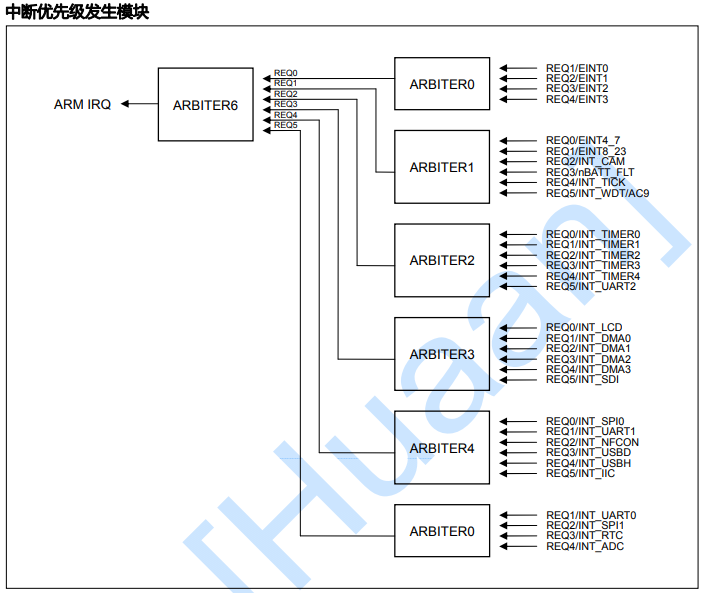
\includegraphics[width=0.6\textwidth]{int2.png}
  \caption{中断优先级}
\end{figure}


\subsubsection{中断服务子程序}
打开\lstinline{interrupt.c},这里是中断服务子程序,我们可以看到
\lstset{language=C}
\begin{lstlisting}{中断服务子程序}
  void EINT_Handle()
  {
      unsigned long oft = INTOFFSET;
      unsigned long val;
      switch( oft )
      {
          // S2被按下
          case 0: 
          {   
              GPFDAT |= (0x7<<4);   // 所有LED熄灭
              GPFDAT &= ~(1<<4);      // LED1点亮
              break;
          }
          
          // S3被按下
          case 2:
          {   
              GPFDAT |= (0x7<<4);   // 所有LED熄灭
              GPFDAT &= ~(1<<5);      // LED2点亮
              break;
          }
          // K4被按下
          case 5:
          {   
              GPFDAT |= (0x7<<4);   // 所有LED熄灭
              GPFDAT &= ~(1<<6);      // LED4点亮                
              break;
          }
          default:
              break;
      }
      //清中断
      if( oft == 5 ) 
          EINTPEND = (1<<11);   // EINT8_23合用IRQ5
      SRCPND = 1<<oft;
      INTPND = 1<<oft;
    //SRCPND = SRCPND;
  }
\end{lstlisting}
这里用到INTOFFSET寄存器,通过读取此寄存器,获得最优先级的中断请求。\\
\\
除此以外还需要把SRCPND和INTPND中的相应的位清零(通过置1来清零),
因为当中断发生时,2440会自动把这两个寄存器中相对应的位置1,以表示某一中断发生,
如果不在中断处理函数内把它们清零,系统会一直执行该中断函数。
另外还是由于前面介绍过的,有一些中断是共用一个中断向量的,
而一个中断向量只能有一个中断执行函数,因此具体是哪个外部中断,
还需要EINTPEND来判断,并同样还要通过置1的方式把相应的位清零。\\

\subsection{结果}
中断点亮小灯
\subsection{问题与总结}
此程序缺乏防抖,容易造成误触,需要进一步开发。
\newpage
\section{双机异步通信查询实现}
\subsection{原理分析}
S3C2440A 的通用异步收发器(UART)配有 3 个独立异步串行 I/O(SIO)端口,
每个都可以是基于中断或基于 DMA 模式的操作。即UART 可以通过产生中断或 DMA 
请求来进行 CPU 和 UART 之间的数据传输。\\
S3C2440A 的 UART 包括了可编程波特率,红外(IR)发送/接收,插入 1 个或 2 
个停止位,5 位、6 位、7 位或 8 位的数据宽度以及奇偶校验。\\
每个 UART 包含一个波特率发生器、发送器、接收器和一个控制单元,
波特率发生器可以由PCLK、FCLK/n 或 UEXTCLK(外部输入时钟)时钟驱动。\\
\\
原理图如下:\\
\begin{figure}[htbp]
  \centering
  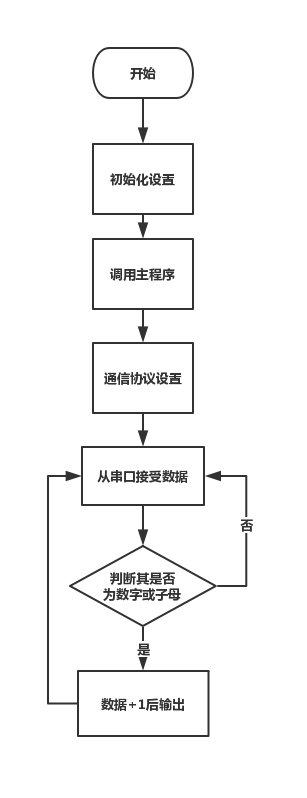
\includegraphics[width=0.3\textwidth]{sch2.png}
  \caption{双机异步通信查询实现原理图}
\end{figure}
\\
\\
\\

\subsection{调试过程}
\subsubsection{uart初始化程序}
head.s程序:\\
功能:初始化,设置clock和把代码搬到sdram快速运行。\\
\lstset{language=bash}
\begin{lstlisting}{初始化程序}
    bl  clock_init          @ 设置MPLL,改变FCLK、HCLK、PCLK
    bl  memsetup            @ 设置存储控制器以使用SDRAM
    bl  copy_steppingstone_to_sdram     @ 复制代码到SDRAM中
\end{lstlisting}
此段代码为初始化的核心,调用了各个初始化函数,如\lstinline{clock_init}。

\subsubsection{uart clock配置}
打开\lstinline{init.c},这里对clock进行配置,我们可以看到
\lstset{language=C}
\begin{lstlisting}{clock配置}
    #define S3C2410_MPLL_200MHZ     ((0x5c<<12)|(0x04<<4)|(0x00))
    #define S3C2440_MPLL_200MHZ     ((0x5c<<12)|(0x01<<4)|(0x02))
    void clock_init(void)
    {
        // LOCKTIME = 0x00ffffff;   // 使用默认值即可
        CLKDIVN  = 0x03;            // FCLK:HCLK:PCLK=1:2:4, HDIVN=1,PDIVN=1

        /* 如果HDIVN非0,CPU的总线模式应该从“fast bus mode”变为“asynchronous bus mode” */
        __asm__(
            "mrc    p15, 0, r1, c1, c0, 0\n"        /* 读出控制寄存器 */ 
            "orr    r1, r1, #0xc0000000\n"          /* 设置为“asynchronous bus mode” */
            "mcr    p15, 0, r1, c1, c0, 0\n"        /* 写入控制寄存器 */
            );

            /* 判断是S3C2410还是S3C2440 */
            if ((GSTATUS1 == 0x32410000) || (GSTATUS1 == 0x32410002))
            {
                MPLLCON = S3C2410_MPLL_200MHZ;  /* 现在,FCLK=200MHz,HCLK=100MHz,PCLK=50MHz */
            }
            else
            {
                MPLLCON = S3C2440_MPLL_200MHZ;  /* 现在,FCLK=200MHz,HCLK=100MHz,PCLK=50MHz */
            }       
    }
\end{lstlisting}
对于MPLLCON寄存器,[19:12]为MDIV,[9:4]为PDIV,[1:0]为SDIV
有如下计算公式:\\
\lstinline{MPLL(FCLK) = (2 * m * Fin)/(p * 2^s)}\\
其中: m = MDIV + 8, p = PDIV + 2, s = SDIV\\
对于本开发板,Fin = 12MHz,设置CLKDIVN,令分频比为:FCLK:HCLK:PCLK=1:2:4,\\
FCLK=200MHz,HCLK=100MHz,PCLK=50MHz

同时,打开\lstinline{interrupt.c},我们可以看到
\lstset{language=C}
\begin{lstlisting}{clock配置}
    ULCON0 &=0XFFFFFF00;
    ULCON0 |=0X03;      // 8N1(8个数据位,无较验,1个停止位)
    ///
    UCON0   = 0x05;     // 查询方式,UART时钟源为PCLK
    ///
    UFCON0  = 0x00;     // 不使用FIFO
    UMCON0  = 0x00;     // 不使用流控
    UBRDIV0 = UART_BRD; // 波特率为115200
\end{lstlisting}
这里把UART时钟源设置为PCLK,并且不使用FIFO,不使用流控,设置波特率为115200。\\
\\
S3C2440A 中的时钟控制逻辑可以产生必须的时钟信号,包括 CPU 的 FCLK,AHB 总线
外设的 HCLK 以及APB 总线外设的 PCLK。S3C2440A 包含两个锁相环(PLL):
一个提供给 FCLK、HCLK 和 PCLK,另一个专用于USB 模块(48MHz)。
时钟控制逻辑可以不使用 PLL 来减慢时钟,并且可以由软件连接或断开各外
设模块的时钟,以降低功耗。\\
\\
其中FCLK,HCLK 和 PCLK的分析如下:\\
FCLK 是提供给 ARM920T 的时钟。\\
HCLK 是提供给用于 ARM920T,存储器控制器,中断控制器,LCD 控制器,DMA 和 USB 主机模块的 AHB
总线的时钟。\\
PCLK 是提供给用于外设如 WDT,IIS,I2C,PWM 定时器,MMC/SD 接口,ADC,UART,GPIO,RTC 和
SPI 的 APB 总线的时钟。\\
S3C2440A 还支持对 FCLK、HCLK 和 PCLK 之间分频比例的选择。该比例由 CLKDIVN 控制寄存器中的 HDIVN
和 PDIVN 所决定。\\
分频比例如下:
\begin{figure}[htbp]
  \centering
  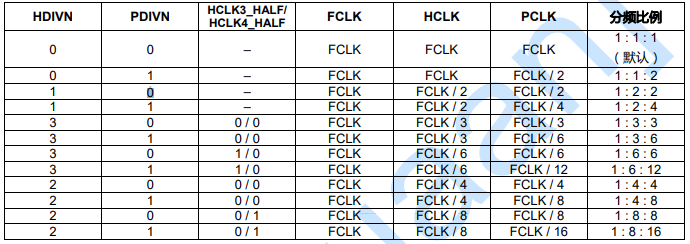
\includegraphics[width=0.8\textwidth]{uart1.png}
  \caption{分频比例}
\end{figure}

\subsubsection{uart循环发送程序}
我们为了能够直观看到结果,将main.c的代码修改成发送机子和接收机子。\\
\\
发送机子主程序:\\
功能:每次复位即向uart0发送a。\\
\lstset{language=bash}
\begin{lstlisting}{发送机子main.c程序}
    int main()
    {
        uart0_init(); 
        unsigned char c='a';
        putc(c);
        return 0;
    }
\end{lstlisting}
接收机子主程序:\\
功能:查询uart0。\\
\lstset{language=bash}
\begin{lstlisting}{接收机子main.c程序}
    int main()
    {
        unsigned char c;
        uart0_init(); 
        while(1)
        {
            c = getc();
            if (isDigit(c) || isLetter(c))
                putc(c+1);
        }
        return 0;
    }
\end{lstlisting}


\subsection{结果}
每次按下发送机子的复位键,接收机子即可接收到“a”。
\begin{figure}[htbp]
    \centering
    
\includegraphics[width=0.8\textwidth]{result0.png}
    \caption{双机异步通信查询实现}
  \end{figure}
\subsection{问题与总结}
1. 原程序无法成功发送,需要自己看懂putc并发送。\\
2. 需要看原理图来查看哪一个管脚是发送,哪一个是接收。
\newpage
\section{异步通信中断发送实现}
把中断点亮小灯和双机异步通信查询实现结合,实现异步通信中断发送实现。
\subsection{原理分析}
在\lstinline{int}的基础上,加入\lstinline{clock_init}等初始化函数配置\lstinline{uart}即可\\
\\
原理图如下:\\
\begin{figure}[htbp]
  \centering
  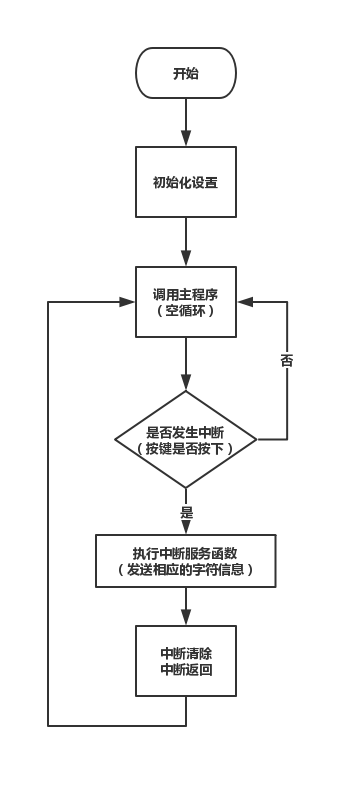
\includegraphics[width=0.3\textwidth]{sch3.png}
  \caption{异步通信中断发送实现原理图}
\end{figure}
\\
\subsection{调试过程}
\subsubsection{初始化程序}
功能:初始化,设置clock和把代码搬到sdram快速运行,并且设置中断模式、
管理模式的栈,设置好中断处理函数。\\
\lstset{language=bash}
\begin{lstlisting}{初始化程序}
    bl  clock_init          @ 设置MPLL,改变FCLK、HCLK、PCLK
    bl  memsetup            @ 设置存储控制器以使用SDRAM
    bl  copy_steppingstone_to_sdram     @ 复制代码到SDRAM中
    bl  init_led            @ 初始化LED的GPIO管脚
    bl  init_irq            @ 调用中断初始化函数,在init.c中
\end{lstlisting}

\subsubsection{中断服务子程序}
打开\lstinline{interrupt.c},这里是中断服务子程序,我们可以看到
\lstset{language=C}
\begin{lstlisting}{中断服务子程序}
    void EINT_Handle()
    {
        unsigned long oft = INTOFFSET;
        unsigned long val;
        unsigned char a='a';
        unsigned char b='b';
        unsigned char c='c';
        uart0_init();   // 波特率115200,8N1(8个数据位,无校验位,1个停止位)
        switch( oft )
        {
            // S2被按下
            case 0: 
            {   
                putc(a);
                break;
            }
            
            // S3被按下
            case 2:
            {   
            putc(b);
                break;
            }
    
            // K4被按下
            case 5:
            {   
                putc(c);             
                break;
            }
            default:
                break;
        }
        if( oft == 5 ) 
            EINTPEND = (1<<11);   // EINT8_23合用IRQ5
        SRCPND = 1<<oft;
        INTPND = 1<<oft;
    }
\end{lstlisting}
当按下对应按键的时候,uart0会发送出"a","b","c"等字母

\subsection{结果}
当按下对应按键的时候,屏幕上会打印出"a","b","c"等字母
\begin{figure}[htbp]
    \centering
    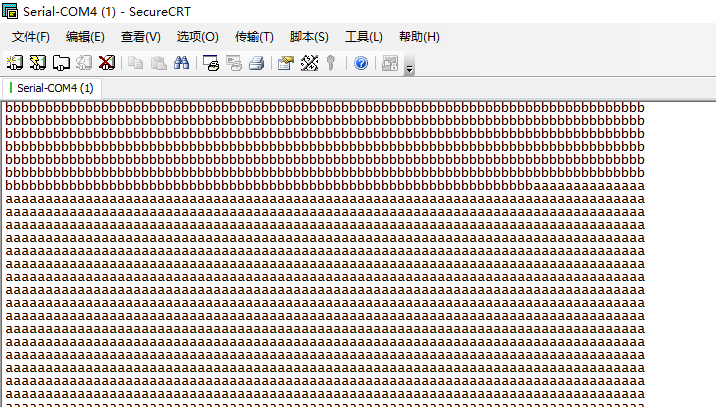
\includegraphics[width=0.8\textwidth]{result1.png}
    \caption{分频比例}
  \end{figure}
\subsection{问题与总结}
中断程序与uart程序结合的时候,可以把一样性质的函数放在一起,不改变函数名,
这样makefile便无需修改。\\
一步一步修改,不可一次改完直接运行,这样的话难以debug。
\newpage
\section{双机异步通信中断发送,查询接收实现}
双机通过中断发送,查询接收实现实现互相通信,并增加小灯以作展示。
\subsection{原理分析}
在异步通信中断发送实现的基础上,加入双机异步通信查询接收\\
\\
原理图如下:\\
\begin{figure}[htbp]
  \centering
  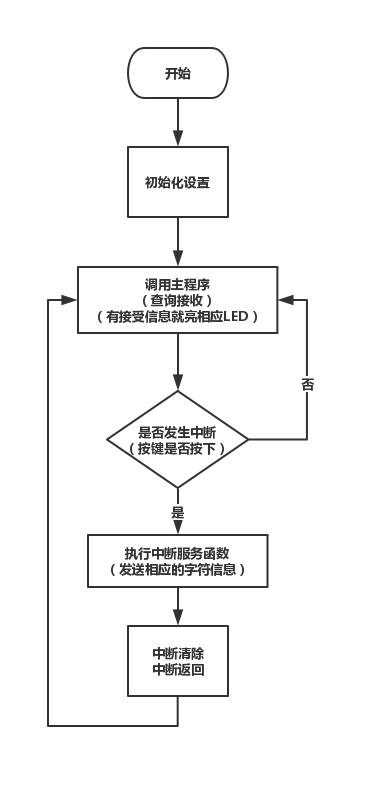
\includegraphics[width=0.3\textwidth]{sch4.png}
  \caption{双机异步通信中断发送,查询接收实现原理图}
\end{figure}
\\
\subsection{调试过程}
\subsubsection{主程序}
\lstset{language=C}
\begin{lstlisting}{主程序}
    int main()
    {
        unsigned char c;
        uart0_init();  
        GPFCON &= ~(GPF4_msk | GPF5_msk | GPF6_msk);
        GPFCON |= GPF4_out | GPF5_out | GPF6_out;
    
        while(1)
        {
            c = getc();
            if (c == 'a'){
                GPFDAT &= ~(1<<4);
                GPFDAT |= (1<<5);
                GPFDAT |= (1<<6);
            } 
            else if (c == 'b'){
                GPFDAT |= (1<<4);
                GPFDAT &= ~(1<<5);
                GPFDAT |= (1<<6);
            }
            else if (c == 'c'){
                GPFDAT |= (1<<4);
                GPFDAT |= (1<<5);
                GPFDAT &= ~(1<<6);
            }
        }
        return 0;
    }
\end{lstlisting}
没有按下按键时,其一直在查询uart0寄存器的数值,若有接收,则点亮对应的灯。
当按下对应按键的时候,uart0会发送出"a","b","c"等字母。


\subsection{结果}
当按下对应按键的时候,对方机子会亮对应的灯,反之亦是。
\begin{figure}[htbp]
    \centering
    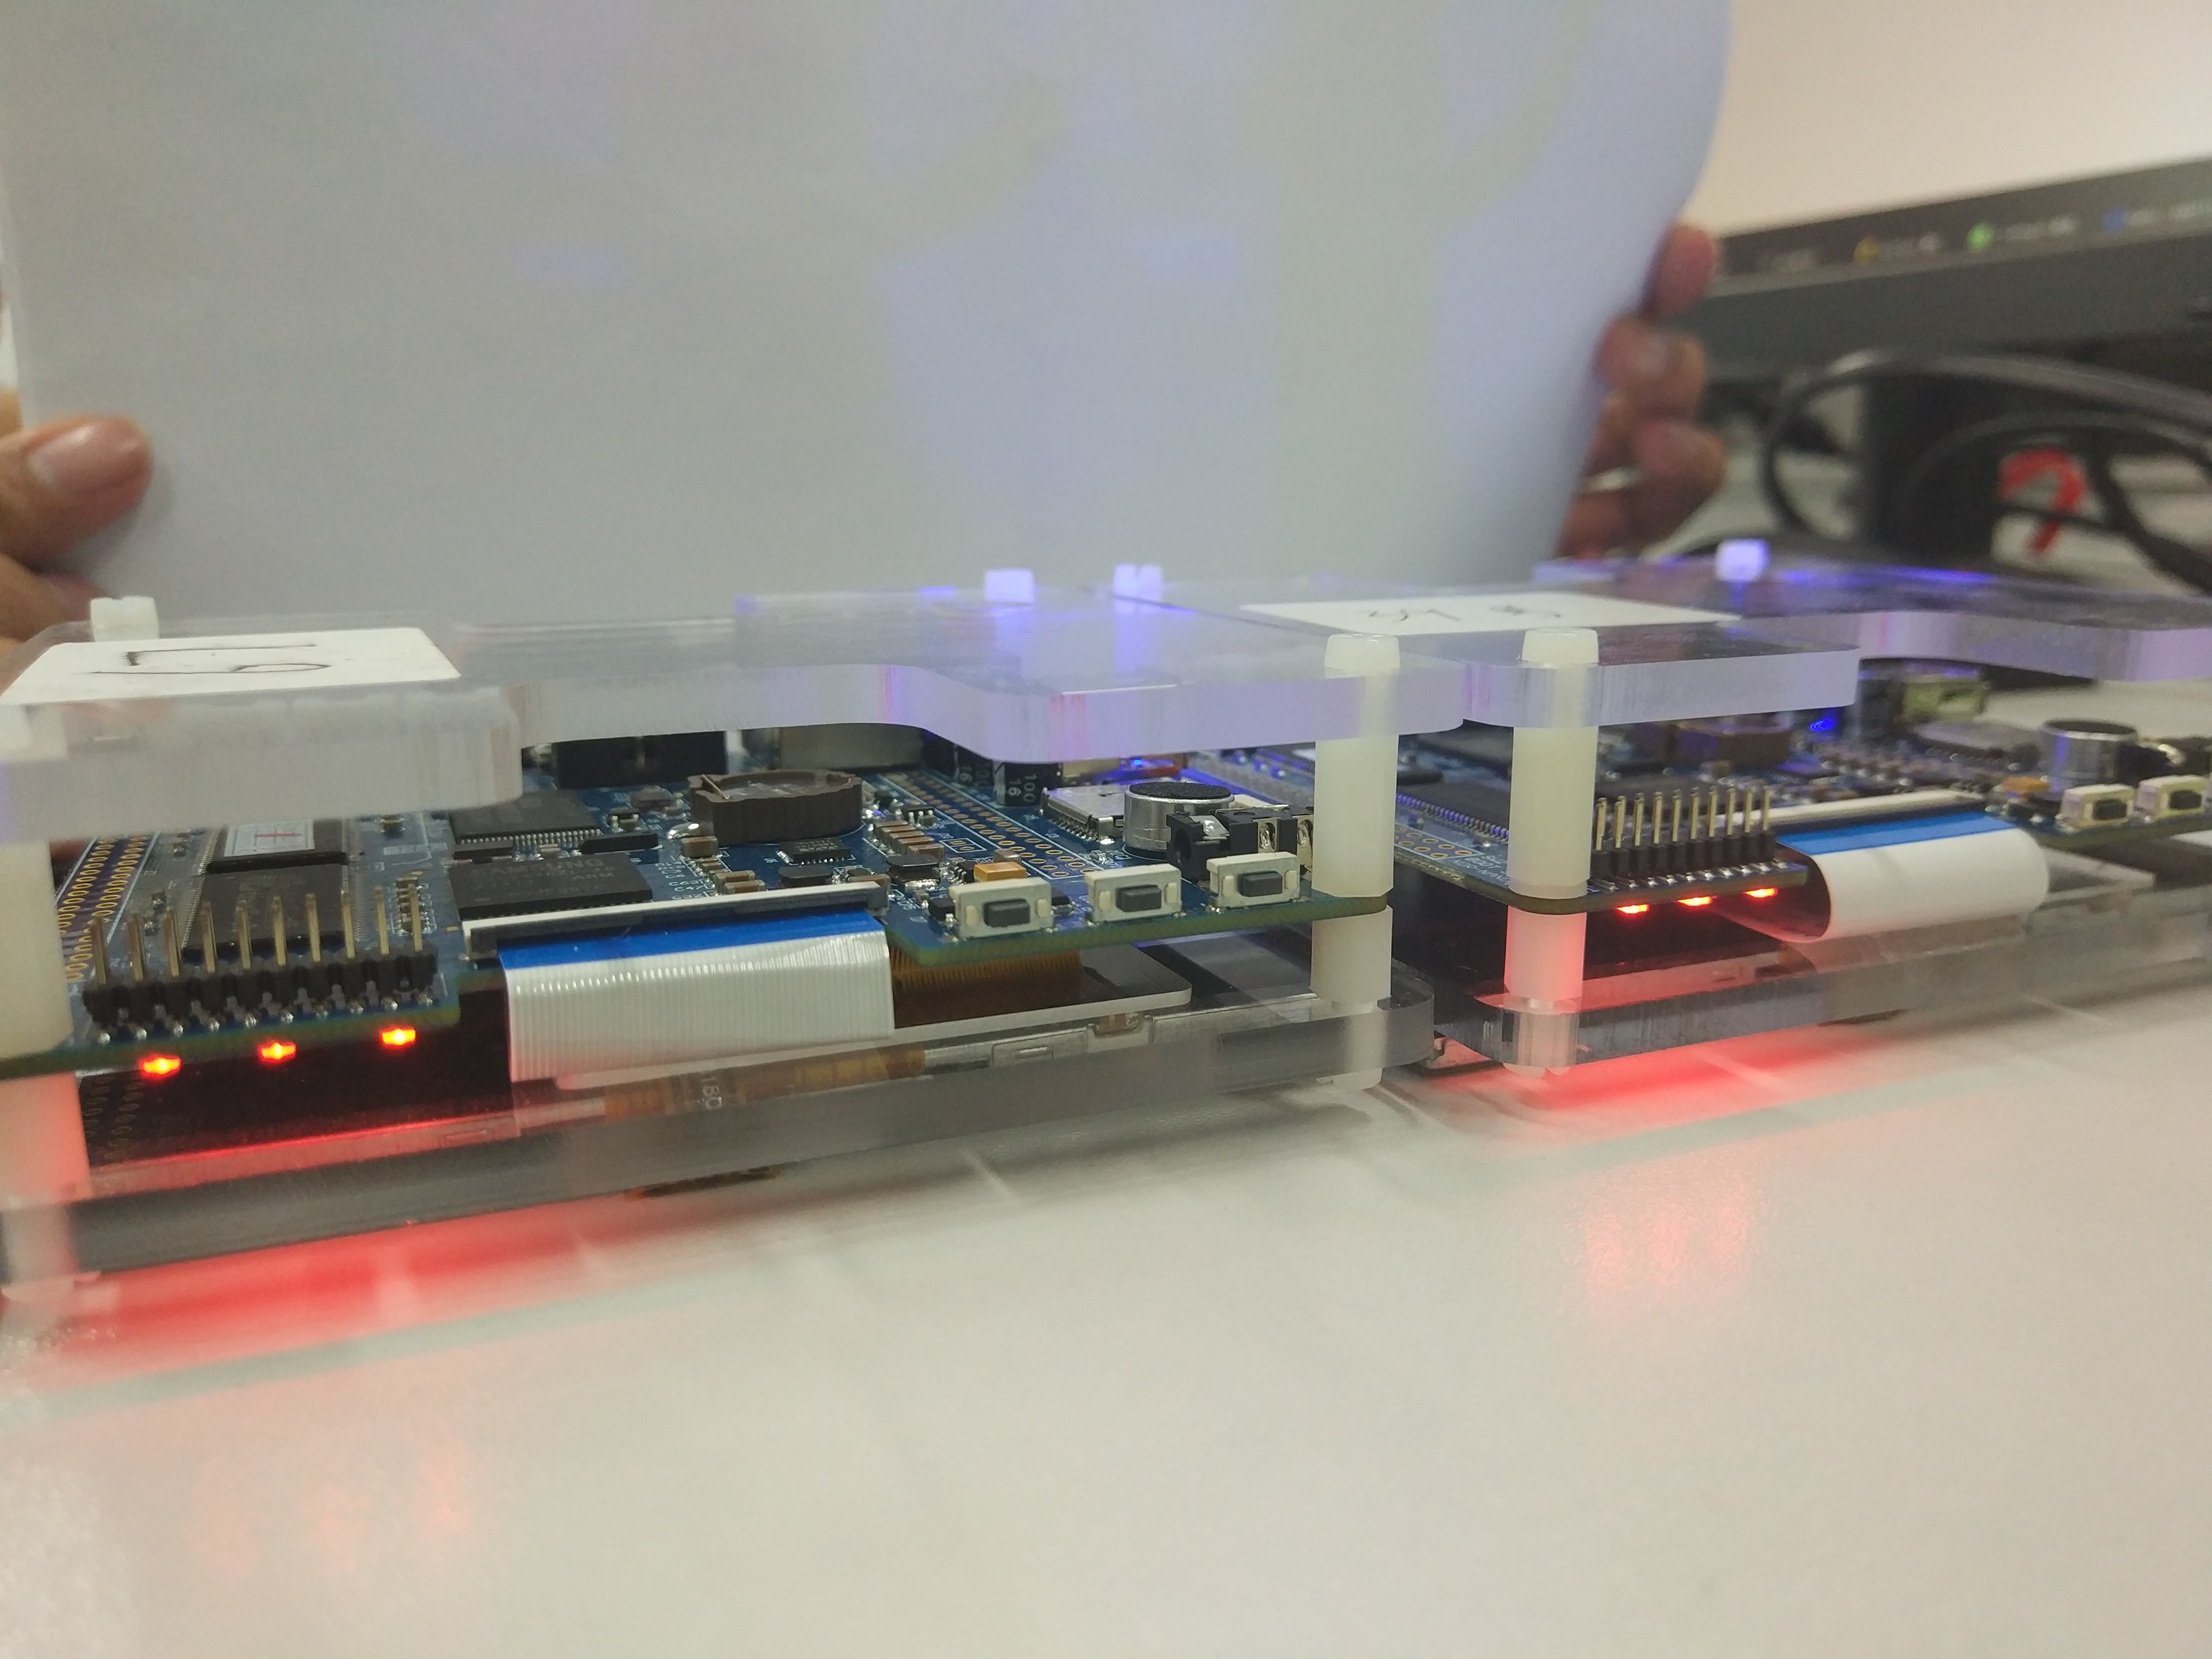
\includegraphics[width=0.5\textwidth]{result4-1}
    \caption{原始状态}
\end{figure}

\begin{figure}[htbp]
    \centering
    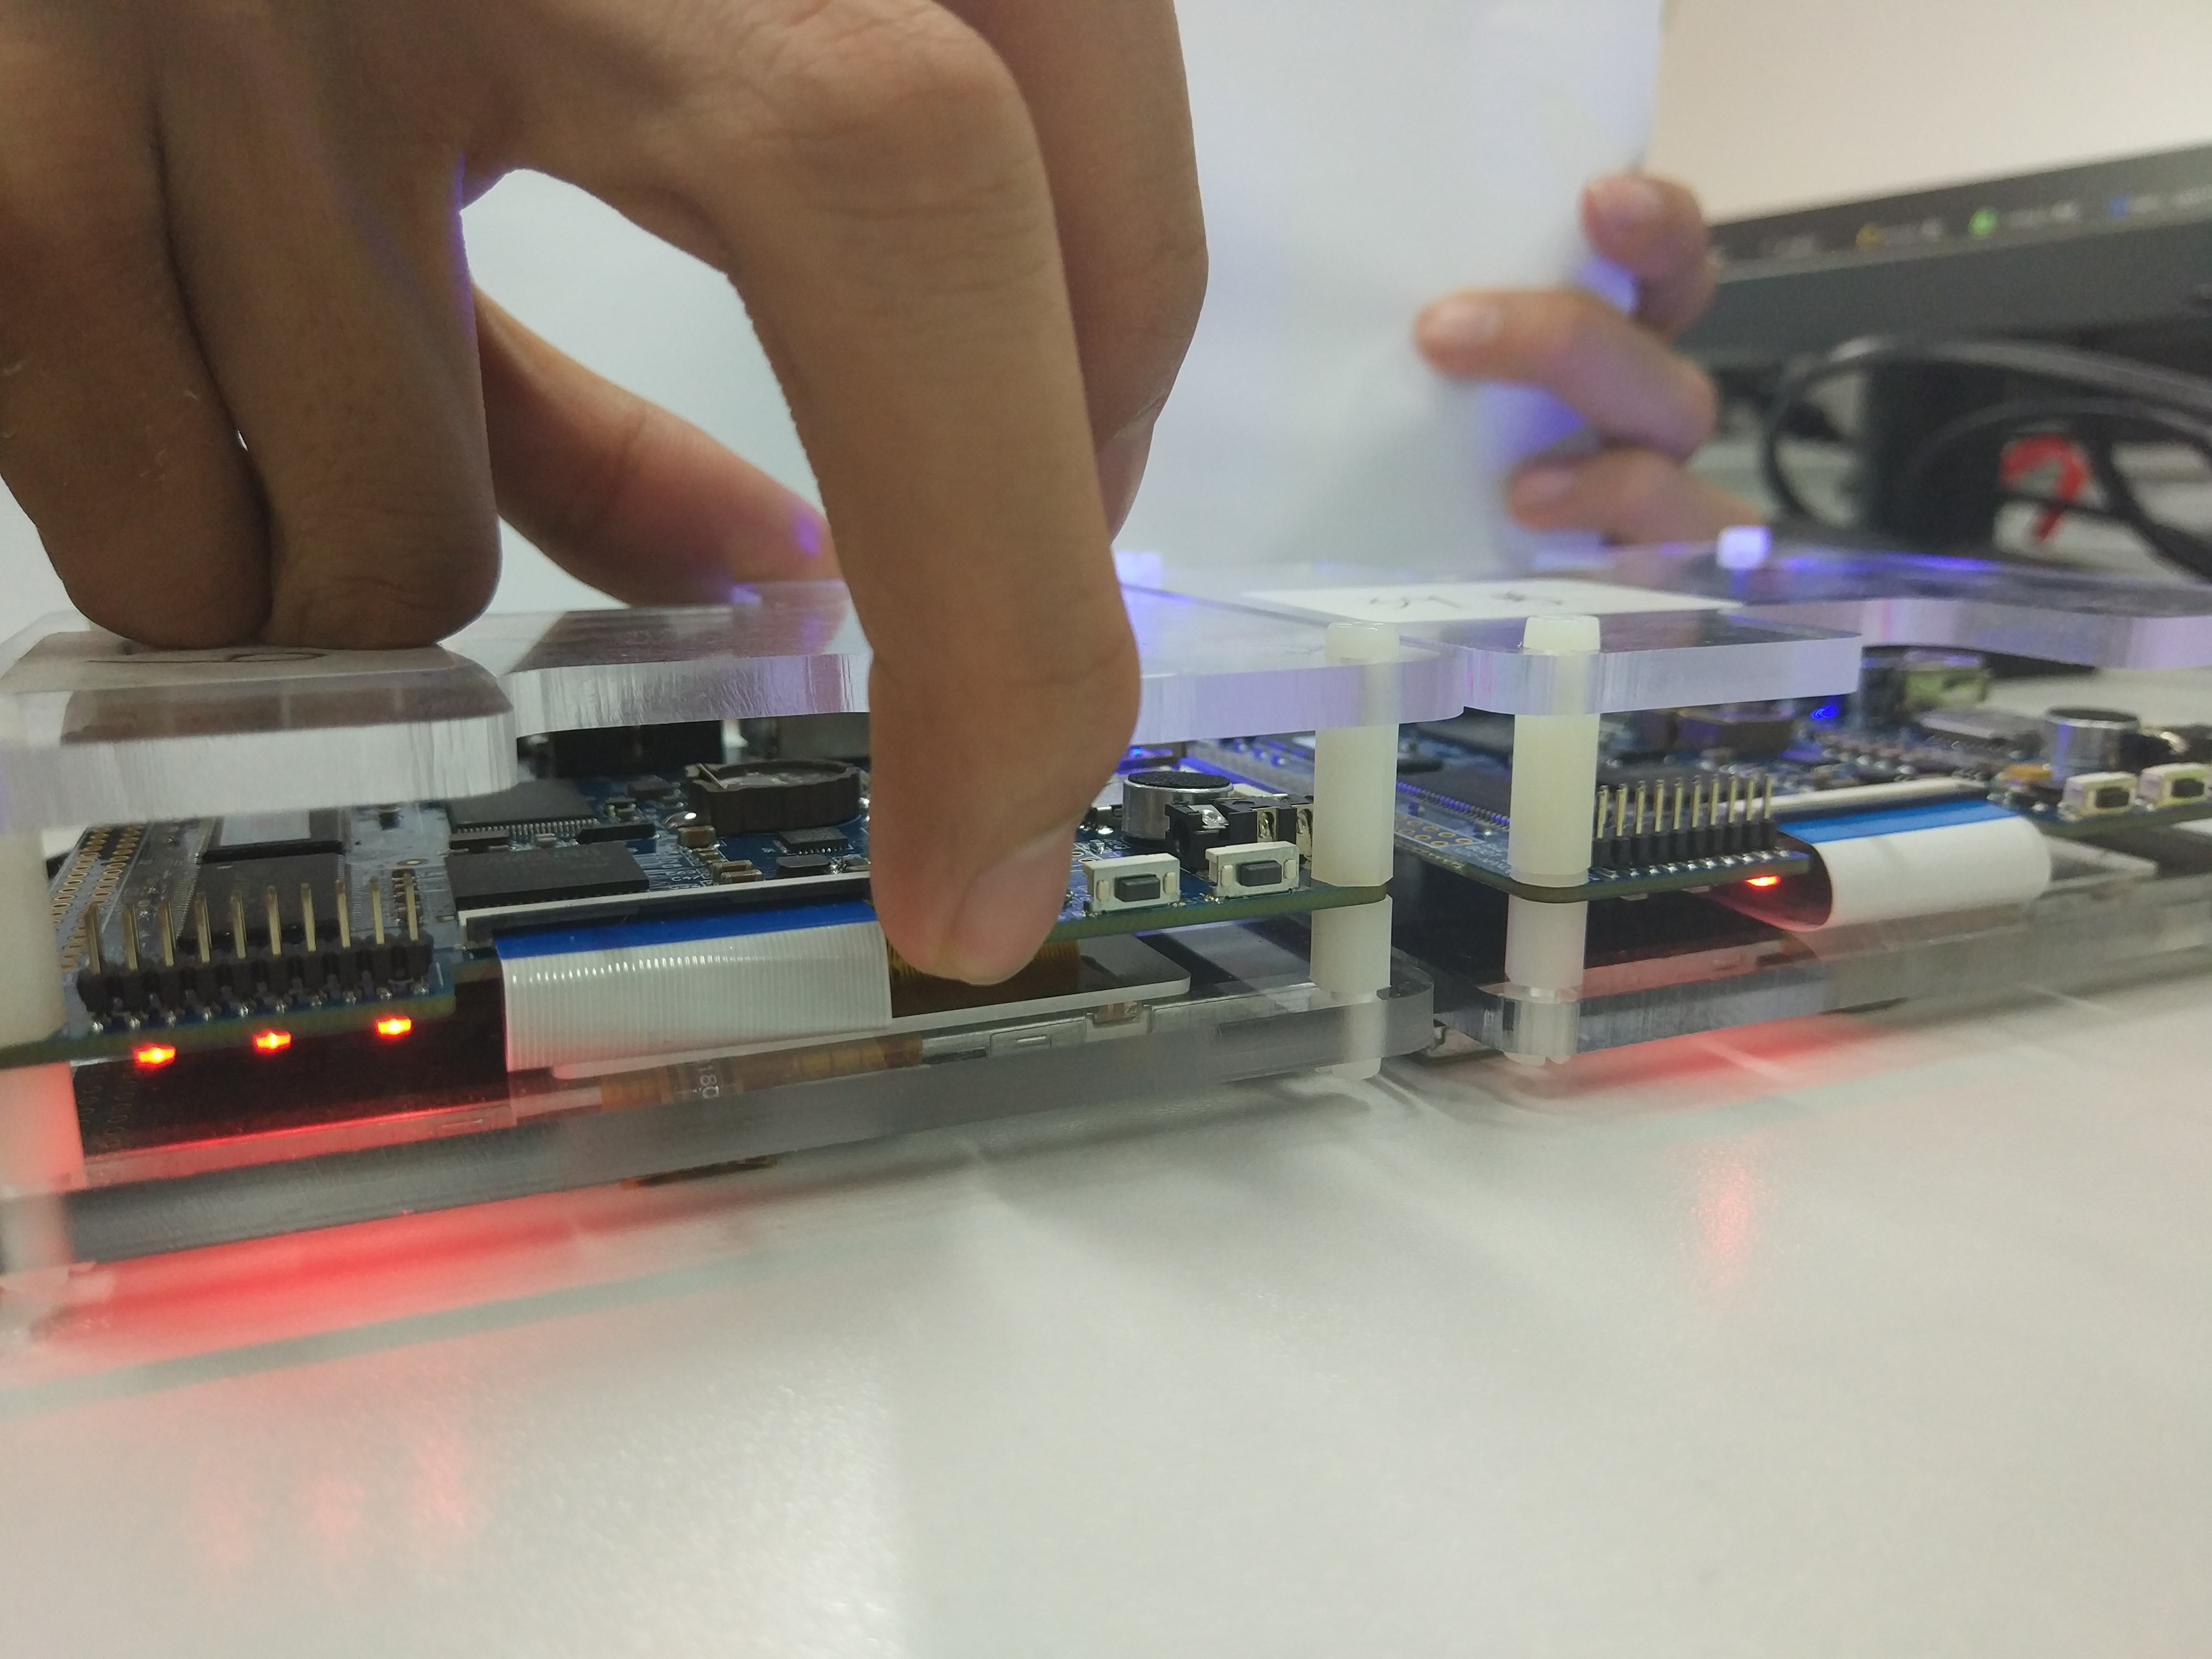
\includegraphics[width=0.5\textwidth]{result4-2}
    \caption{按下1号机子}
\end{figure}

\begin{figure}[htbp]
    \centering
    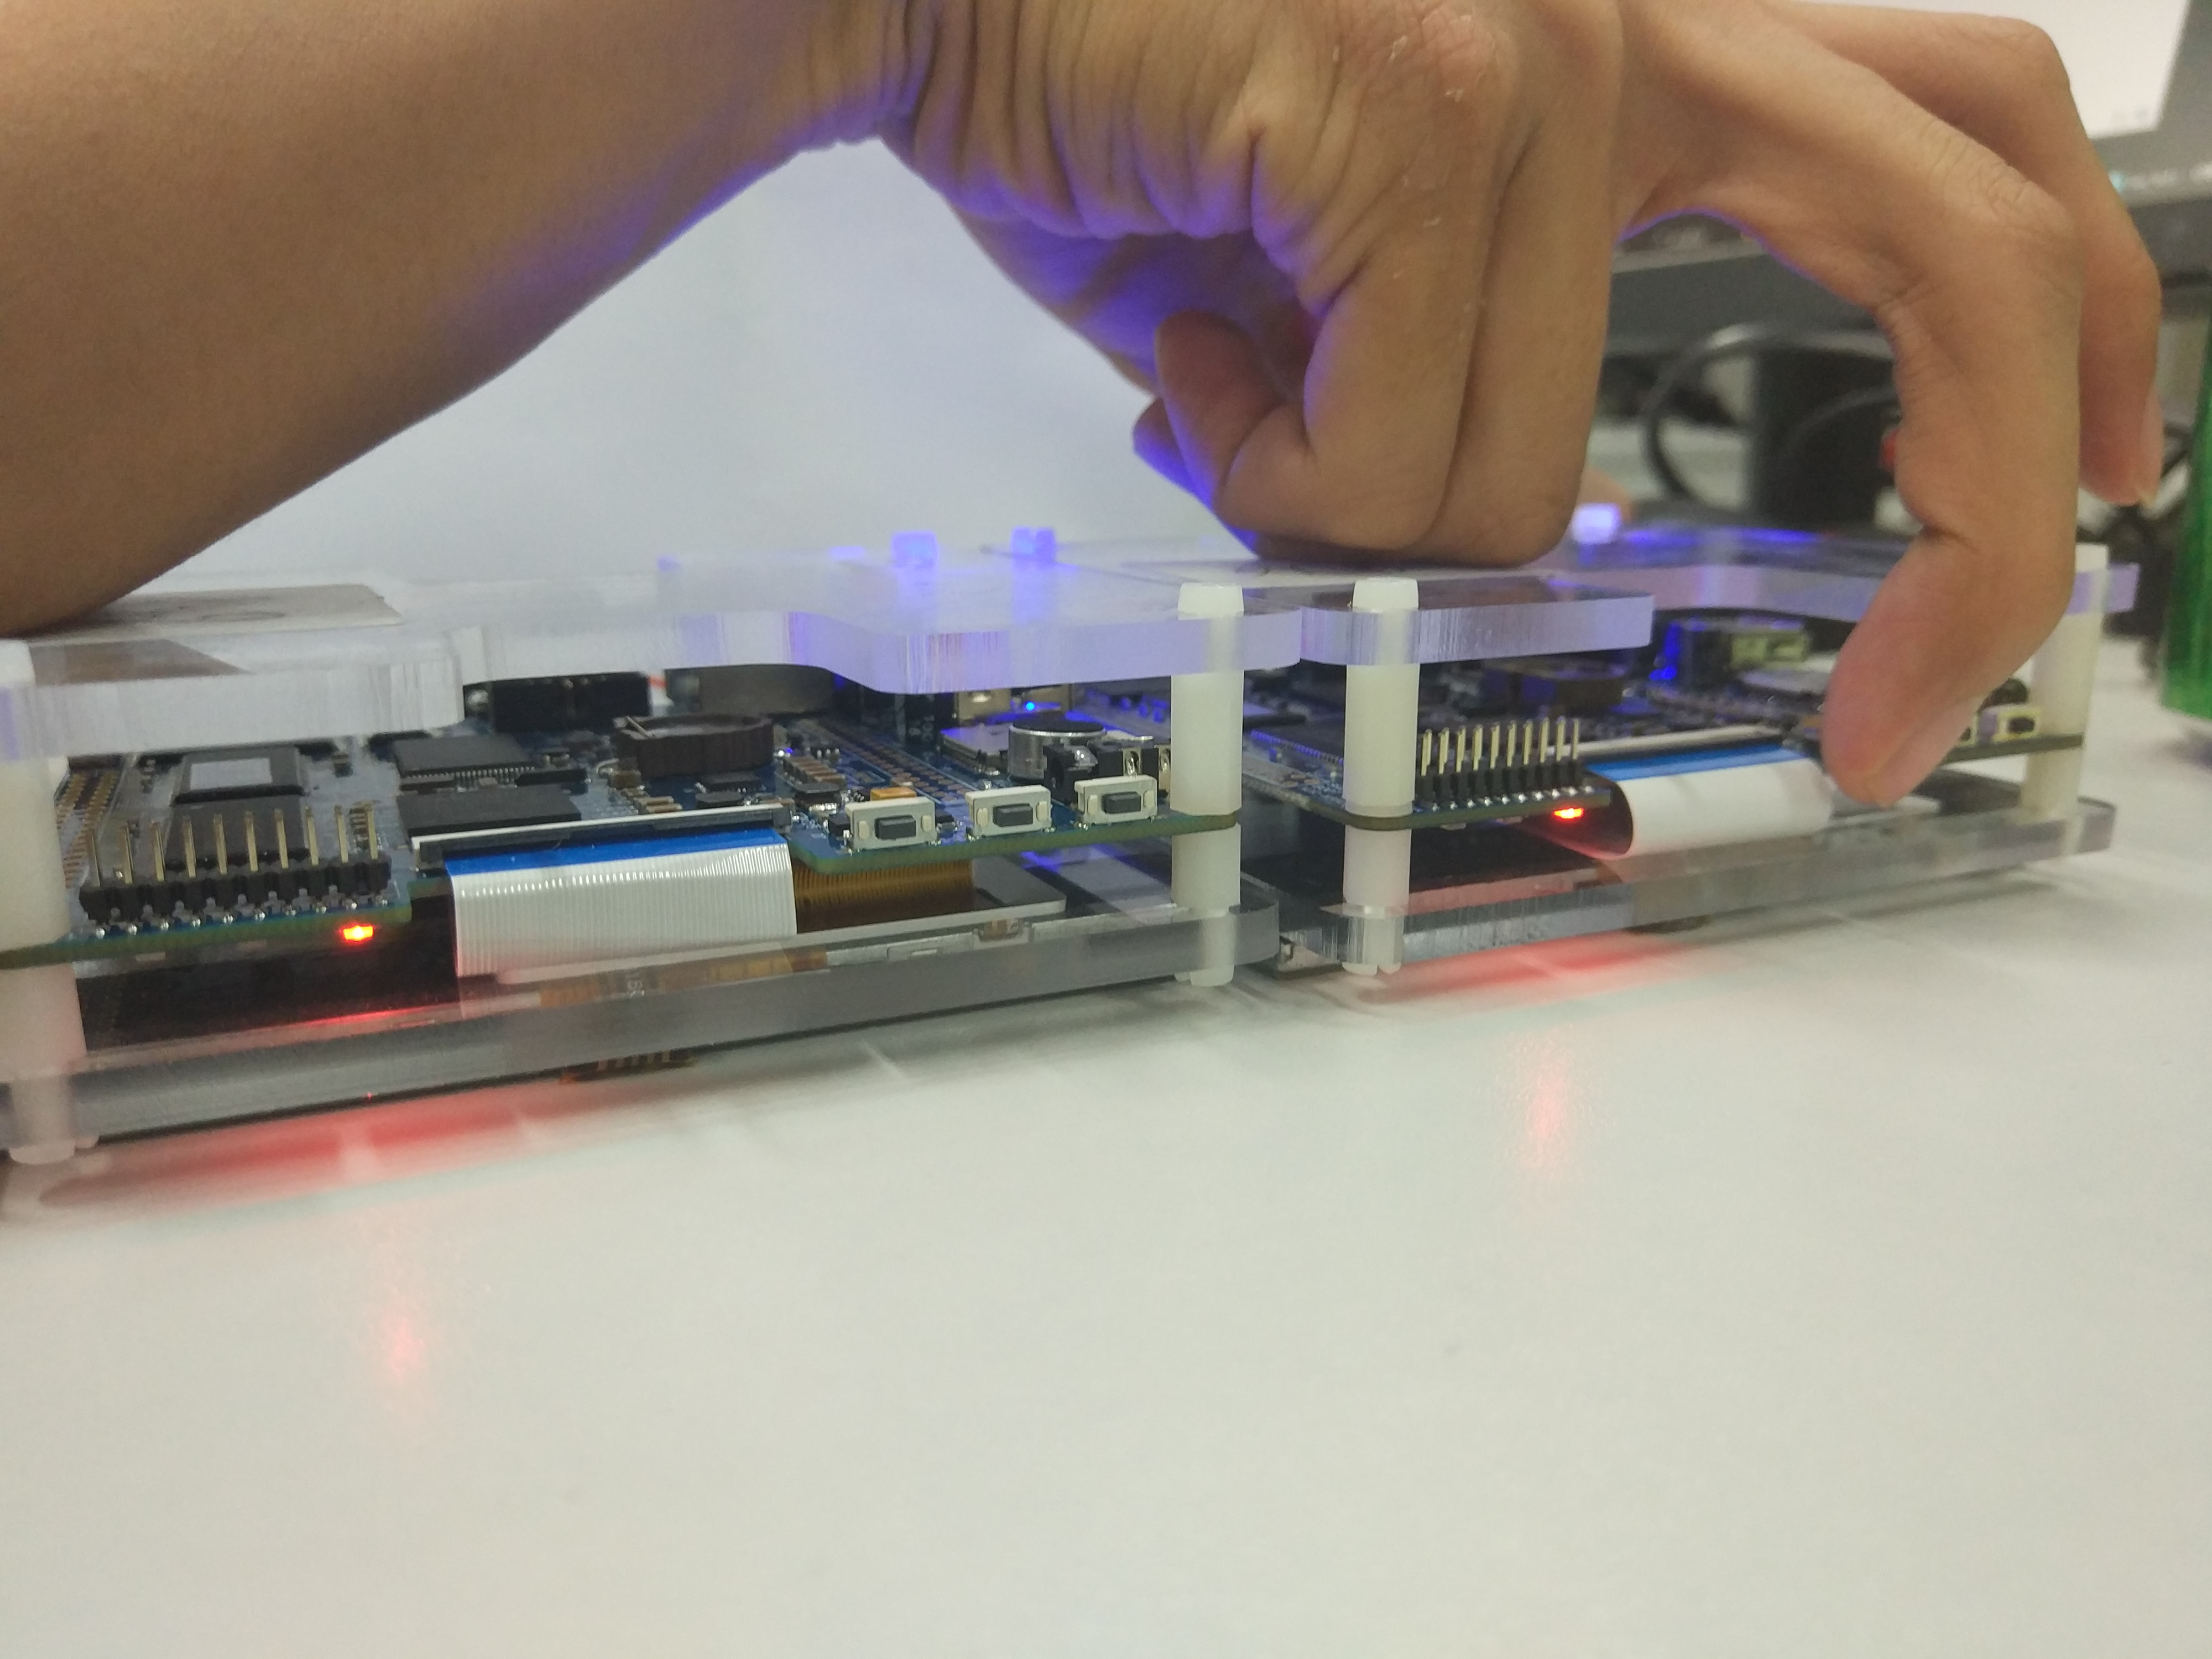
\includegraphics[width=0.5\textwidth]{result4-3}
    \caption{按下2号机子}
\end{figure}
\subsection{问题与总结}
使用的是查询接收,效率不高,需进一步改进。
\newpage
\section{异步通信中断接收实现}
一台机子使用中断发送,一台机子使用中断接收。
\subsection{原理分析}
在异步通信中断发送实现的基础上,打开uart0的中断,以用于中断接收,并用led来展示。\\
\\
原理图如下:\\
\begin{figure}[htbp]
  \centering
  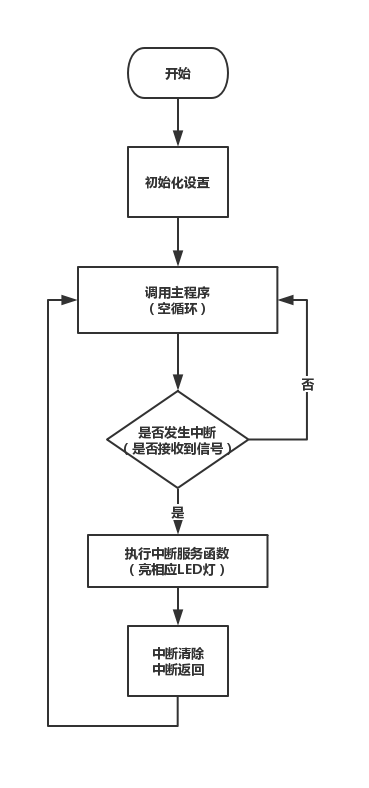
\includegraphics[width=0.3\textwidth]{sch5.png}
  \caption{异步通信中断接收实现原理图}
\end{figure}
\\

\subsection{调试过程}
\subsubsection{UART寄存器分析}
打开\lstinline{s3c24xx.h},这里使用到的interrupt registes,我们可以看到
\lstset{language=C}

\begin{lstlisting}{UART寄存器分析}
    /*UART registers*/
    #define ULCON0              (*(volatile unsigned long *)0x50000000)
    #define UCON0               (*(volatile unsigned long *)0x50000004)
    #define UFCON0              (*(volatile unsigned long *)0x50000008)
    #define UMCON0              (*(volatile unsigned long *)0x5000000c)
    #define UTRSTAT0            (*(volatile unsigned long *)0x50000010)
    #define UTXH0               (*(volatile unsigned char *)0x50000020)
    #define URXH0               (*(volatile unsigned char *)0x50000024)
    #define UBRDIV0             (*(volatile unsigned long *)0x50000028)
    
\end{lstlisting}
这里使用了大量UART相关寄存器,后面会详细分析。

\subsubsection{UART寄存器配置}
打开\lstinline{init.c},这里对中断寄存器配置,我们可以看到
\lstset{language=C}
\begin{lstlisting}{中断寄存器配置}
    void init_irq( )
    {
        SUBSRCPND |= 0x3;
        SRCPND |= 0x1<<28;
        INTPND |= 0x1<<28;
    
        INTSUBMSK &= ~(0x1);
        INTSUBMSK |= (0x1<<1);
        INTMSK &= ~(0x1<<28);
    }
\end{lstlisting}

\lstset{language=C}
\begin{lstlisting}{中断寄存器配置}
    void uart0_init(void)
    {
        GPHCON&=0x3c0000;
        GPHCON|=0x2faaa;
        GPBCON = 0x1dd7fc;//GPB5,6,8,10设置为输出
        GPBDAT|=0x560;//4个LED全灭
        GPHUP=0x1ff;//H口上拉禁止
        GPFCON &=~((3<<0)|(3<<4)|(3<<6)|(3<<8)) ;
        GPFCON |= ((2<<0)|(2<<4)|(2<<6)|(2<<8)) ;//GPF0,GPF2,GPF3,GPF4工作在第二功能状态,即中断
        EINTPEND=(1<<4);
    
        
        ULCON0 &=0XFFFFFF00;
        ULCON0 |=0X03;      // 8N1(8个数据位,无较验,1个停止位)
        UCON0   = 0x09;     // 中断请求
        UFCON0  = 0x00;     // 不使用FIFO
        UMCON0  = 0x00;     // 不使用流控
        UBRDIV0 = UART_BRD; // 波特率为115200
    }

\end{lstlisting}
配置分析:
UART 线路控制寄存器: \\
我们选取8个数据位,无较验,1个停止位\\
 \begin{figure}[h]
    \centering
    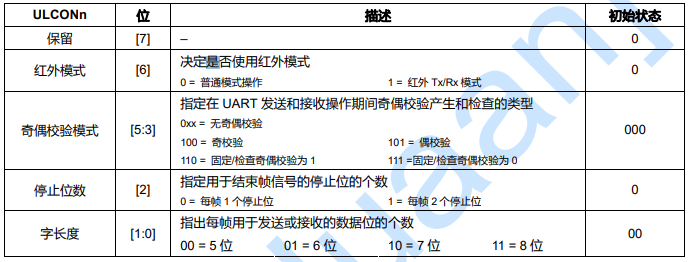
\includegraphics[width=0.7\textwidth]{uart2.png}
    \caption{ULCON0}
\end{figure}
UART 控制寄存器: \\
选取1 = 电平(当非 FIFO 模式中 Tx 缓冲器为空或 FIFO 模式中达到 Tx FIFO 触发深度时请
求中断),并且UFCON0寄存器中,不使用FIFO。UMCON0中,不使用流控。\\
\begin{figure}[h]
    \centering
    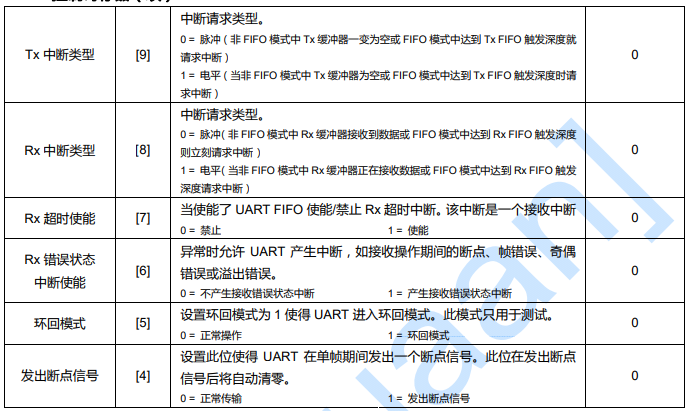
\includegraphics[width=0.7\textwidth]{uart3.png}
    \caption{UCON0}
\end{figure}
\\
我们还要打开对应的中断允许寄存器,
\lstinline{INTMSK &= ~(0x1<<28)};
\begin{figure}[h]
    \centering
    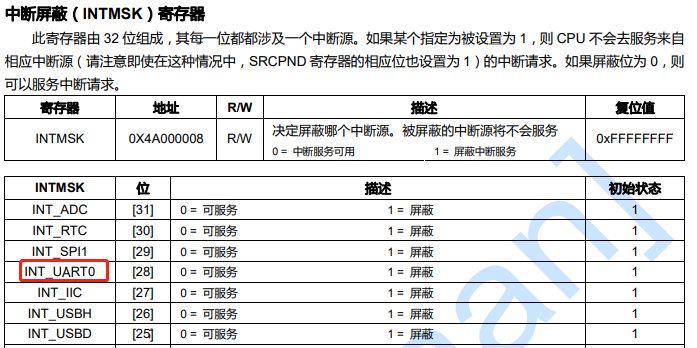
\includegraphics[width=0.7\textwidth]{uart4.png}
    \caption{INTMSK}
\end{figure}
\\
同时,由于我们还要定义是接收还是发送,也要打开INTSUBMSK,\\
\lstinline{INTSUBMSK &= ~(0x1);INTSUBMSK |= (0x1<<1);}
\begin{figure}[h]
    \centering
    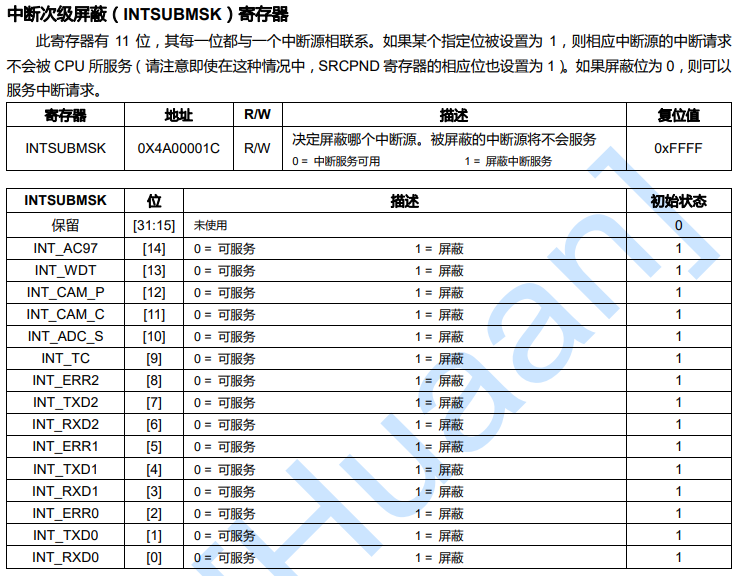
\includegraphics[width=0.7\textwidth]{uart5.png}
    \caption{INTSUBMSK}
\end{figure}

\subsection{结果}
当按下对应按键的时候,对方机子会亮对应的灯。
\begin{figure}[htbp]
    \centering
    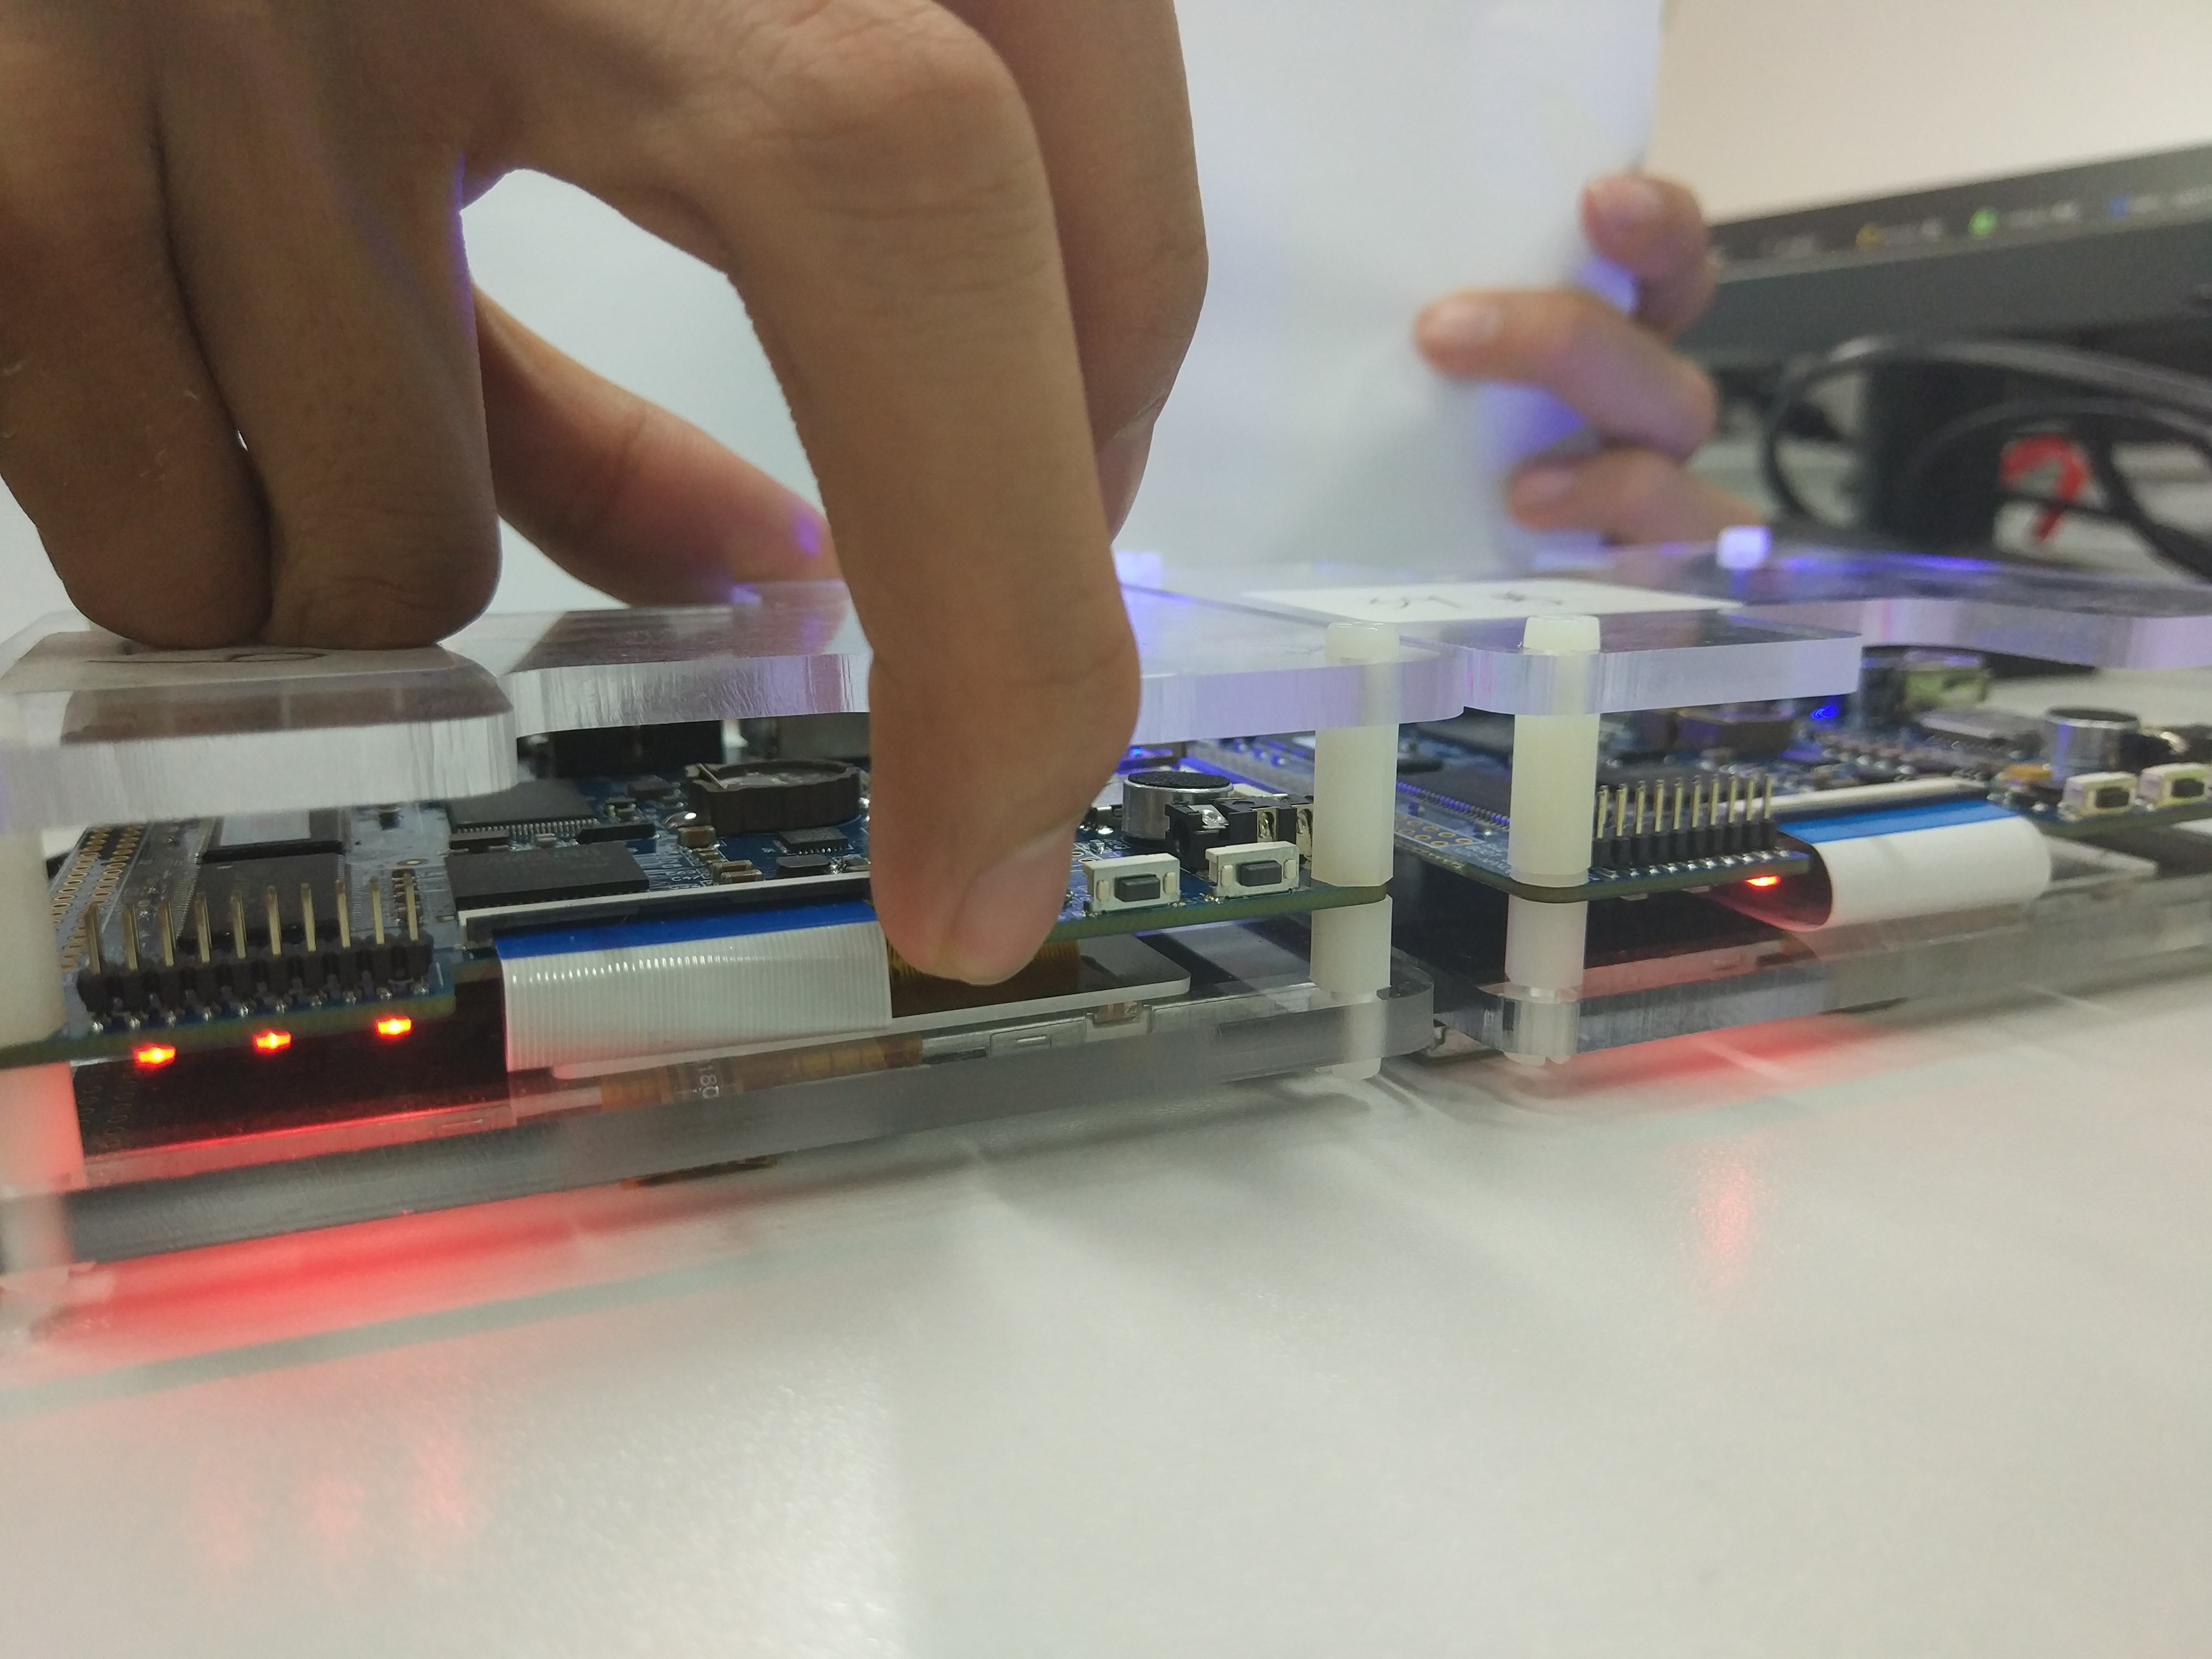
\includegraphics[width=0.5\textwidth]{result4-2}
    \caption{按下1号机子}
\end{figure}
\subsection{问题与总结}
仍然没能把两个中断写在同一个程序内,需要进一步改进。




\end{document}
